\subsection{Kennzahlen}
    Nach jeder Klassifizierung wurden eine Kennzahlen anhand des
    resultierenden Graphens in der Datenbank ermittelt.
    Dies geschah sowohl für die einzelnen Datenbanken
    als auch der gemeinsamen.
    Die folgenden Tabellen sind daher folgendermaßen aufgebaut:
    Die erste Spalte beschreibt die Kennzahl.
    Dann folgen vier Spalten, die den Wert der Kennzahl für die einzelnen Sites enthalten
    Anschließend für jede Kennzahl die Summe der Site-Wert präsentiert.
    Diese kann mit der letzten Spalte verglichen werden,
    die den Wert der Kennzahl für den Fall,
    dass sich alle Klassifikationen in einer Datenbank befinden, enthält.

    Eine ausführliche Interpretation dieser Zahlen geschieht in Kapitel \ref{section:findingsInterpretation}.
    Trotzdem wird auch hier schon die Bedeutung einiger Kennzahlen kurz hervorgehoben.

    Zur besseren Verständnis der präsentierten Kennzahlen,
    veranschaulichen Abbildung
    \ref{image:findingTeachersFiguresDbModel1}
    und \ref{image:findingTeachersFiguresDbModel2},
    wie der Graph der Klassifikation aufgebaut ist.
    Beide sind durch den Content Knoten mit der Klasse "`Teacher"' verbunden.
    Verzichtet wird auf die Darstellung von Referenzen,
    da diese lediglich Kanten von den dargestellten Content Knoten
    zu Resource Knoten sind.
    Welche Content Klassen welche Referenzen besitzen können,
    ist zusammen mit dem Klassifikationsmodell ersichtlich.

    \begin{figure}[htb]
        \centering
        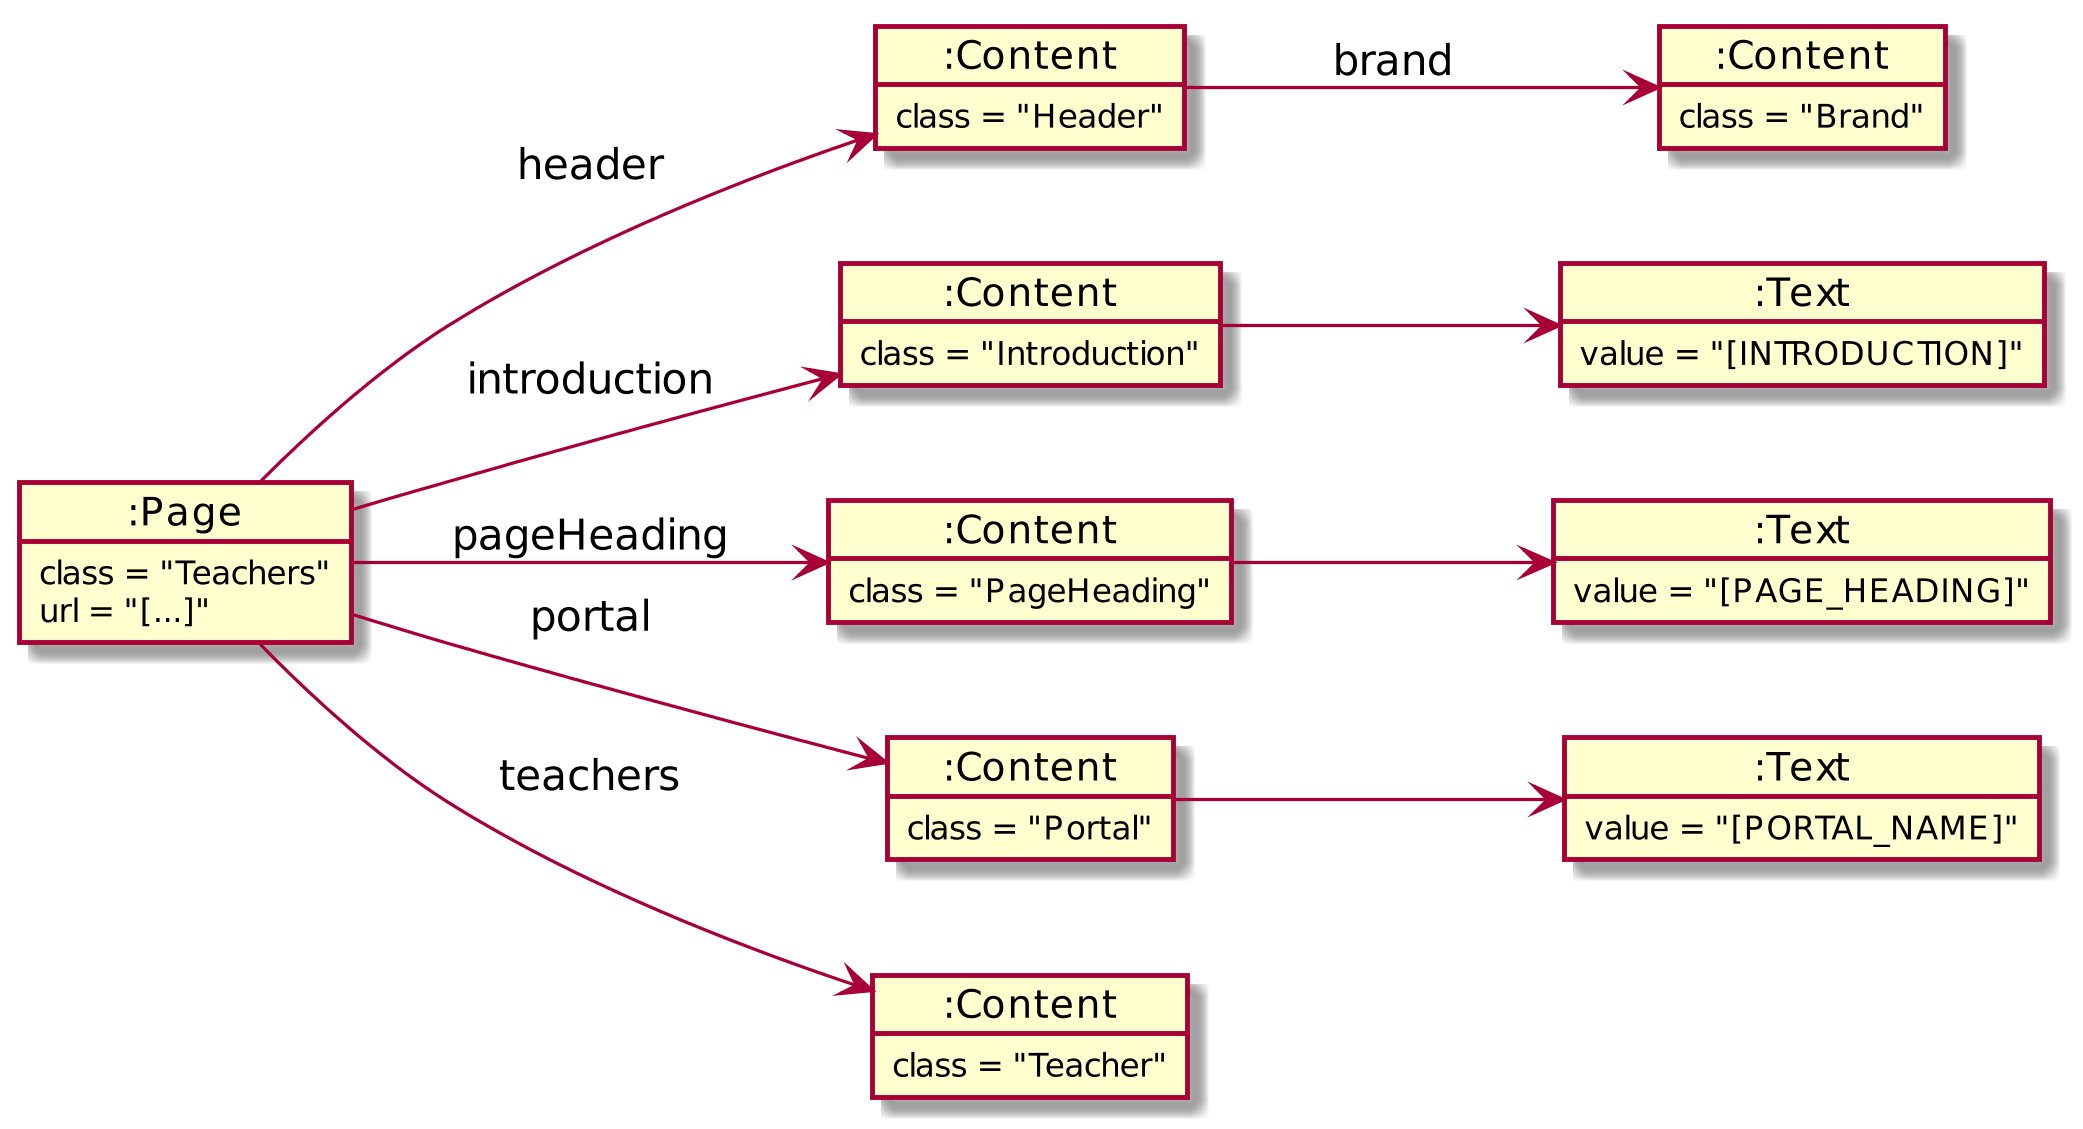
\includegraphics[scale=\imageScalingFactor]{../resources/findings/case-study-1/dbmodel/dbmodel1.png}
        \caption{DB Model 1}
        \label{image:findingTeachersFiguresDbModel1}
    \end{figure}

    \begin{figure}[htb]
        \centering
        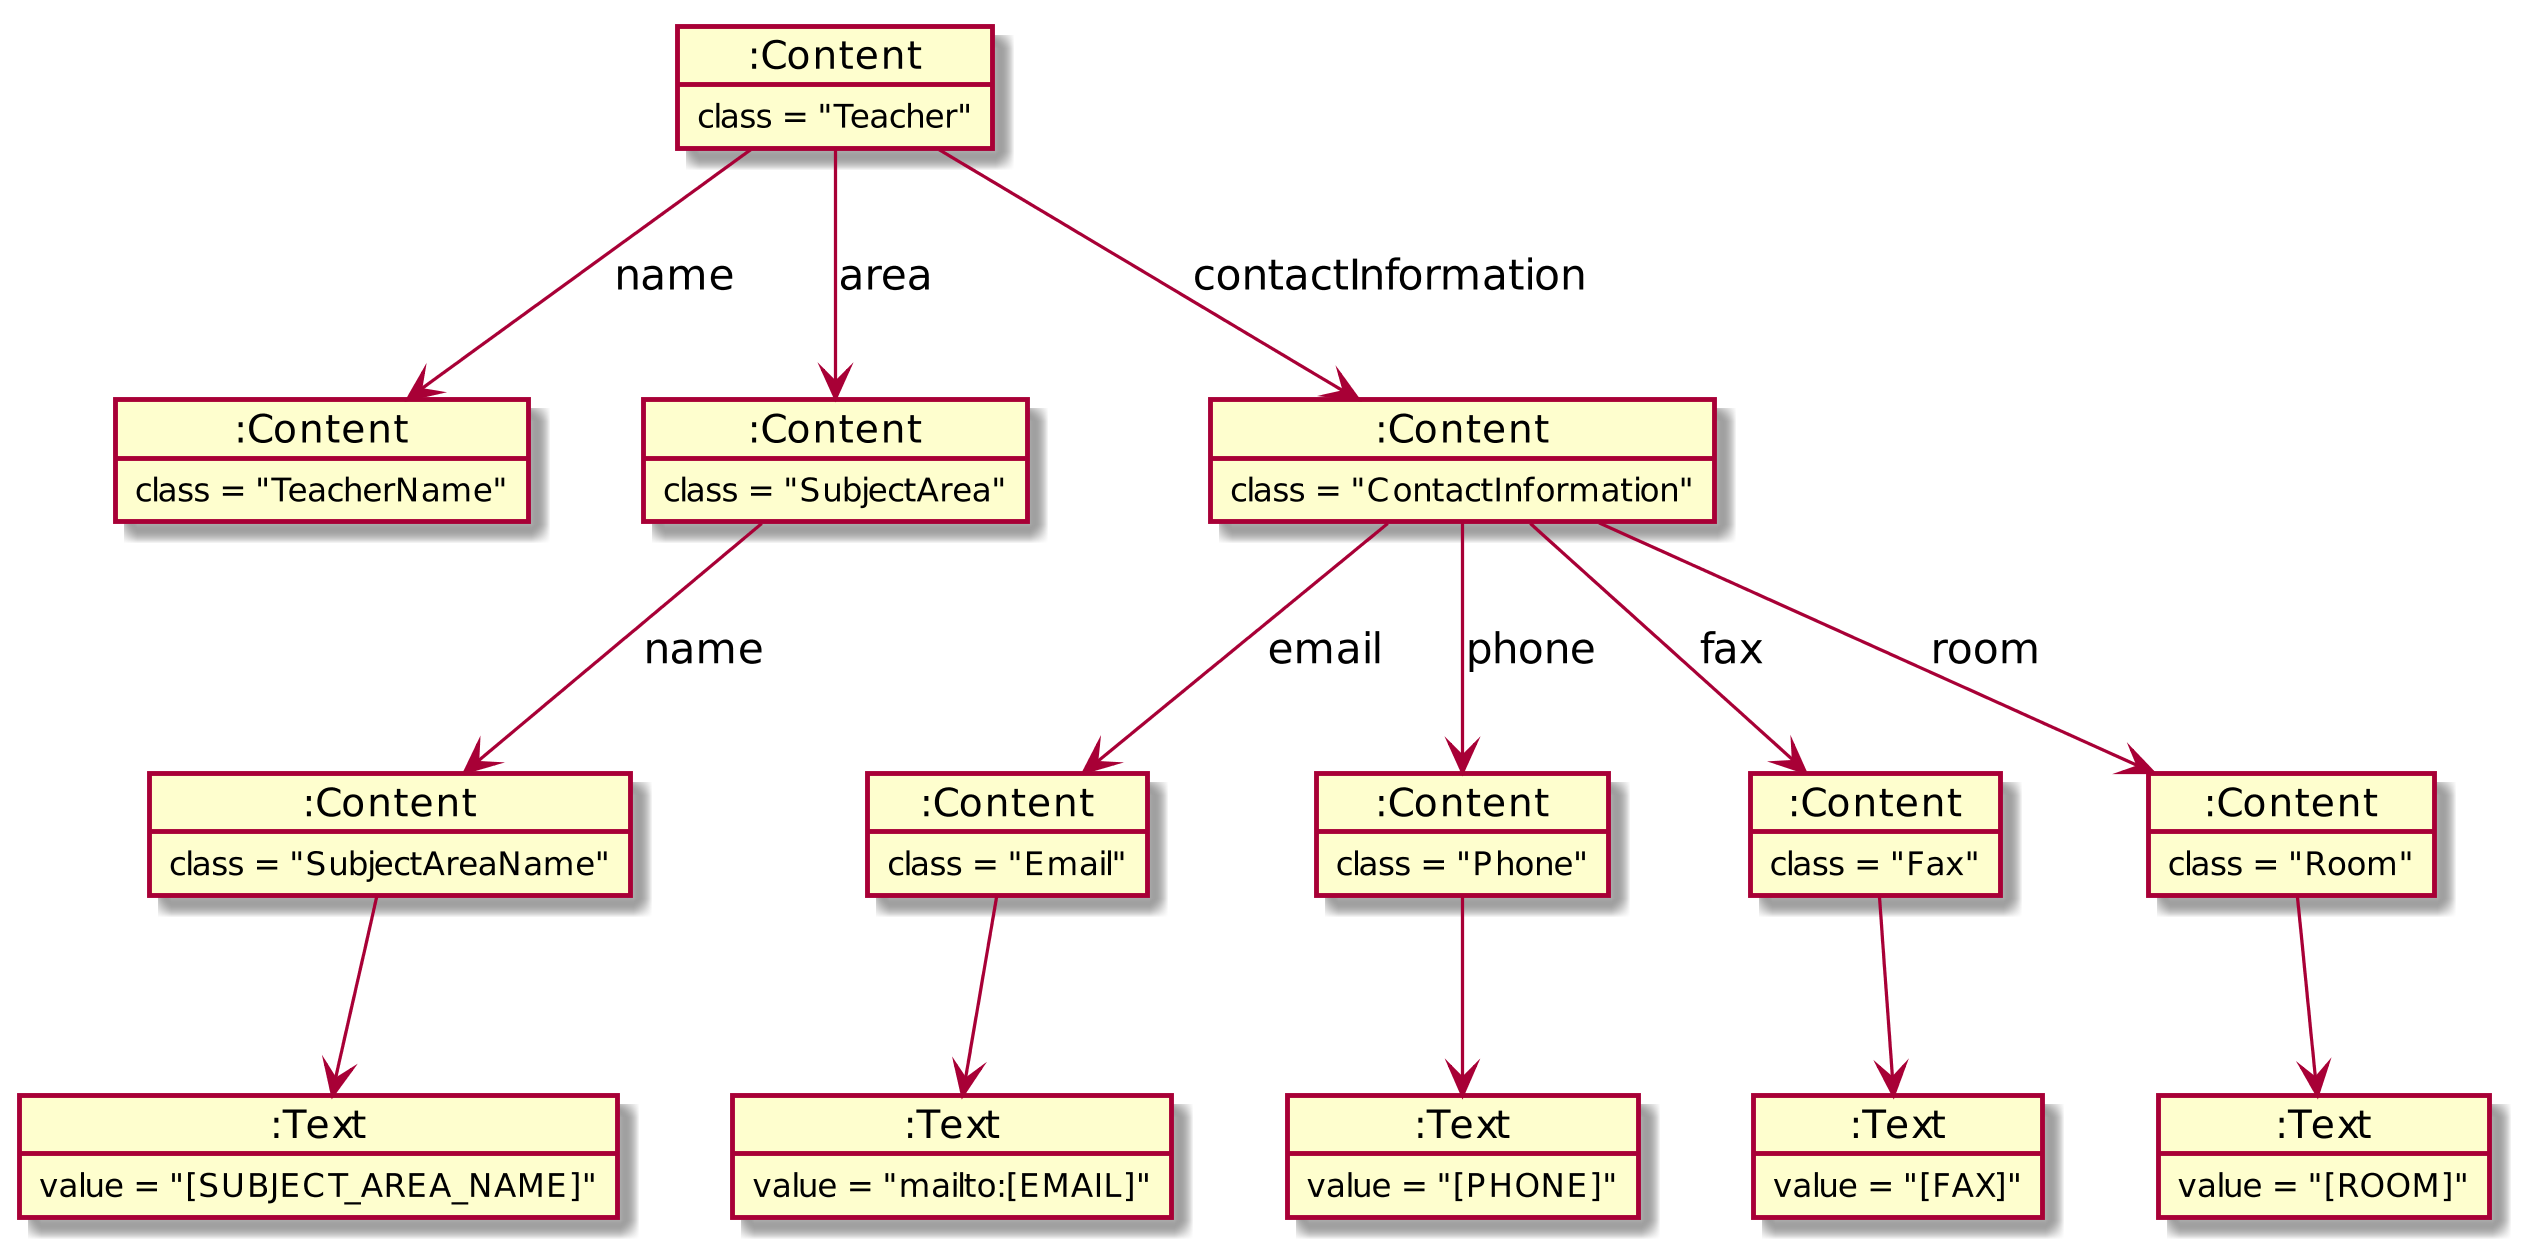
\includegraphics[scale=\imageScalingFactor]{../resources/findings/case-study-1/dbmodel/dbmodel2.png}
        \caption{DB Model 2}
        \label{image:findingTeachersFiguresDbModel2}
    \end{figure}

    Tabelle \ref{table:findingsTeachersFiguresNodesByLabel}
    zeigt wie oft die verschiedenen Labels für Knoten verwendet wurden.
    Die Kennzahl "`Content"' ist in diesem Fall gleichzusetzen mit
    der Anzahl der Content Features in der Klassifikation.

    \begin{table}[htb]
        \centering
        \begin{tabular}{|l|c|c|c|c|c|c|}
            \hline
            \multicolumn{1}{|c|}{\textbf{Label}} & \textbf{BaBw} & \textbf{BaPVS} & \textbf{BscPsy} & \textbf{MaBm} & \textbf{Summe} & \textbf{Alle} \\ \hline
            Content                                     & 270           & 275            & 176             & 128           & 849            & 824           \\ \hline
            Page + Resource                             & 1             & 1              & 1               & 1             & 4              & 4             \\ \hline
            Resource                                    & 133           & 159            & 89              & 71            & 452            & 430           \\ \hline
            Site                                        & 1             & 1              & 1               & 1             & 4              & 4             \\ \hline
            Text                                        & 105           & 69             & 75              & 56            & 305            & 284           \\ \hline
            \hline
            \textbf{Summe}                              & 510           & 505            & 342             & 257           & 1614           & 1546          \\ \hline
        \end{tabular}
        \caption{Anzahl der Knoten nach Label}
        \label{table:findingsTeachersFiguresNodesByLabel}
    \end{table}

    Die Knoten mit dem Label "`Content"' lassen sich nach der ihnen zugewiesenen Klasse
    weiter aufschlüssen, was in Tabelle \ref{table:findingsTeachersFiguresContentNodesByClass} geschieht.
    Eine Kennzahl in dieser Tabelle ist demnach gleichzusetzen mit der Häufigkeit der Verwendung
    der genannten Klasse in der Klassifikation.

    \begin{table}[htb]
        \centering
        \begin{tabular}{|l|c|c|c|c|c|c|}
        \hline
            \textbf{Klasse}  & \multicolumn{1}{l|}{\textbf{BaBw}} & \multicolumn{1}{l|}{\textbf{BaPVS}} & \multicolumn{1}{l|}{\textbf{BscPsy}} & \multicolumn{1}{l|}{\textbf{MaBm}} & \multicolumn{1}{l|}{\textbf{Summe}} & \multicolumn{1}{l|}{\textbf{Alle}} \\ \hline
            Brand              & 1                                  & 1                                   & 1                                    & 1                                  & 4                                   & 4                                  \\ \hline
            ContactInformation & 55                                 & 67                                  & 33                                   & 24                                 & 179                                 & 178                                \\ \hline
            Fax                & 1                                  & 0                                   & 0                                    & 1                                  & 2                                   & 1                                  \\ \hline
            Header             & 1                                  & 1                                   & 1                                    & 1                                  & 4                                   & 4                                  \\ \hline
            Introduction       & 1                                  & 0                                   & 1                                    & 1                                  & 3                                   & 2                                  \\ \hline
            PageHeading        & 1                                  & 1                                   & 1                                    & 1                                  & 4                                   & 4                                  \\ \hline
            Phone              & 35                                 & 38                                  & 29                                   & 21                                 & 123                                 & 119                                \\ \hline
            Portal             & 1                                  & 1                                   & 1                                    & 1                                  & 4                                   & 4                                  \\ \hline
            Room               & 2                                  & 0                                   & 0                                    & 0                                  & 2                                   & 2                                  \\ \hline
            SubjectArea        & 53                                 & 67                                  & 33                                   & 22                                 & 175                                 & 172                                \\ \hline
            SubjectAreaName    & 9                                  & 18                                  & 11                                   & 7                                  & 45                                  & 39                                 \\ \hline
            Teacher            & 55                                 & 70                                  & 33                                   & 24                                 & 182                                 & 182                                \\ \hline
            TeacherName        & 55                                 & 11                                  & 32                                   & 24                                 & 122                                 & 113                                \\ \hline
            \hline
            \textbf{Summe}     & 270                                & 275                                 & 176                                  & 128                                & 849                                 & 824                                \\ \hline
        \end{tabular}
        \caption{Content Knoten aufgeteilt nach Klasse}
        \label{table:findingsTeachersFiguresContentNodesByClass}
    \end{table}

    Auch über die Kanten des Graphens lassen sich eine Zahlen ermitteln.
    Tabelle \ref{table:findingTeachersFiguresEdgesByLabel} beginnt dazu
    mit der Aufschlüsselung der Kanten nach ihrem Label.
    Die Kennzahl "`References"' spiegelt die Anzahl der Referenzen innerhalb der Klassifikation wieder.

    \begin{table}[htb]
        \centering
        \begin{tabular}{|l|c|c|c|c|c|c|}
            \hline
            \multicolumn{1}{|c|}{\textbf{Kanten-Label}} & \textbf{BaBw} & \textbf{BaPVS} & \textbf{BscPsy} & \textbf{MaBm} & \textbf{Summe} & \textbf{Alle} \\ \hline
            Reads                                       & 105           & 69             & 75              & 56            & 305            & 284           \\ \hline
            References                                  & 180           & 209            & 110             & 86            & 585            & 582           \\ \hline
            Owns                                        & 320           & 335            & 200             & 144           & 999            & 996           \\ \hline
            \hline
            \textbf{Summe}                              & 605           & 613            & 385             & 286           & 1889           & 1862          \\ \hline
        \end{tabular}
        \caption{Kanten nach Label}
        \label{table:findingTeachersFiguresEdgesByLabel}
    \end{table}

    Neben dem Label ist in Bezug auf Kanten auch die Frage interessant,
    welche Knoten sie verbinden.
    Tabelle \ref{table:findingsTeachersFiguresEdgesByStartEndNodeLabel}
    zeigt, welche Arten von Knoten wie oft verbunden wurden.
    Die Beziehung eines Content Knotens zu einem Text-Knoten ist nicht enthalten,
    da diese äquivalent zum oben gezeigten Reads-Label ist.
    Diese Tabelle liefert unter anderem Informationen darüber,
    wie viele Referenzen die Seite selbst hat und wie viele zu Content Features gehören.

    \begin{table}[htb]
        \centering
        \begin{tabular}{|l|c|c|c|c|c|c|}
            \hline
            \multicolumn{1}{|c|}{\textbf{Start-, Zielknoten-Label}} & \textbf{BaBw} & \textbf{BaPVS} & \textbf{BscPsy} & \textbf{MaBm} & \textbf{Summe} & \textbf{Alle} \\ \hline
            (:Content) $\rightarrow$ (:Content)                           & 260           & 260            & 162             & 115           & 797            & 794           \\ \hline
            (:Content) $\rightarrow$ (:Resource)                         & 172           & 201            & 102             & 78            & 553            & 550           \\ \hline
            (:Page) $\rightarrow$ (:Content)                              & 59            & 74             & 37              & 28            & 198            & 198           \\ \hline
            (:Page) $\rightarrow$ (:Resource)                             & 8             & 8              & 8               & 8             & 32             & 32            \\ \hline
            (:Site) $\rightarrow$ (:Page)                                 & 1             & 1              & 1               & 1             & 4              & 4             \\ \hline
            \hline
            \textbf{Summe}                                          & 500           & 544            & 310             & 230           & 1584           & 1578          \\ \hline
        \end{tabular}
        \caption{Kanten nach Start und Zielknoten}
        \label{table:findingsTeachersFiguresEdgesByStartEndNodeLabel}
    \end{table}

    Eine letzte zu beantwortende Frage ist,
    wie viele Knoten in der Datenbank mehr als eine eingehende Kante haben,
    d.h., wie oft sie an verschiedenen Stellen einer oder mehrerer Klassifikationen Verwendung finden.

    \begin{table}[htb]
        \centering
        \begin{tabular}{|l|c|c|c|c|c|c|}
            \hline
            \multicolumn{1}{|c|}{\textbf{Knoten}} & \textbf{BaBw} & \textbf{BaPVS} & \textbf{BscPsy} & \textbf{MaBm} & \textbf{Summe} & \textbf{Alle} \\ \hline
            Bild                                  & 0             & 1              & 1               & 0             & 2              & 2             \\ \hline
            ContactInformation                    & 0             & 3              & 0               & 0             & 3              & 3             \\ \hline
            E-Mail-Adresse                        & 0             & 1              & 1               & 0             & 2              & 14            \\ \hline
            Fax                                   & 0             & 0              & 0               & 0             & 0              & 1             \\ \hline
            Hauptseite "`Studium"'                & 1             & 0              & 0               & 0             & 1              & 1             \\ \hline
            Homepage der FU                       & 0             & 0              & 0               & 0             & 0              & 1             \\ \hline
            Introduction                          & 0             & 0              & 0               & 0             & 0              & 1             \\ \hline
            Lehrgebietsseiten                     & 7             & 16             & 8               & 5             & 36             & 30            \\ \hline
            Phone                                 & 4             & 1              & 0               & 0             & 5              & 9             \\ \hline
            SubjectArea                           & 0             & 2              & 0               & 0             & 2              & 5             \\ \hline
            SubjectAreaName                       & 8             & 16             & 7               & 5             & 36             & 31            \\ \hline
            Teacher                               & 0             & 1              & 0               & 0             & 1              & 1             \\ \hline
            TeacherName                           & 0             & 3              & 1               & 0             & 4              & 13            \\ \hline
            \hline
            \textbf{Summe}                        & 20            & 44             & 18              & 10            & 92             & 112           \\ \hline
        \end{tabular}
        \caption{Mehrfach referenzierte Knoten}
        \label{table:findingsTeachersFiguresSharedNodes}
    \end{table}
